\subsection{Figures}

Results often have figures, but in this case \cref{fig:real_fig} is the only
real figure. There may also be supplementary figures (e.g.,
\cref{fig:supplemental}).

\begin{figure}
    \begin{subfigure}{0.22\textwidth}
        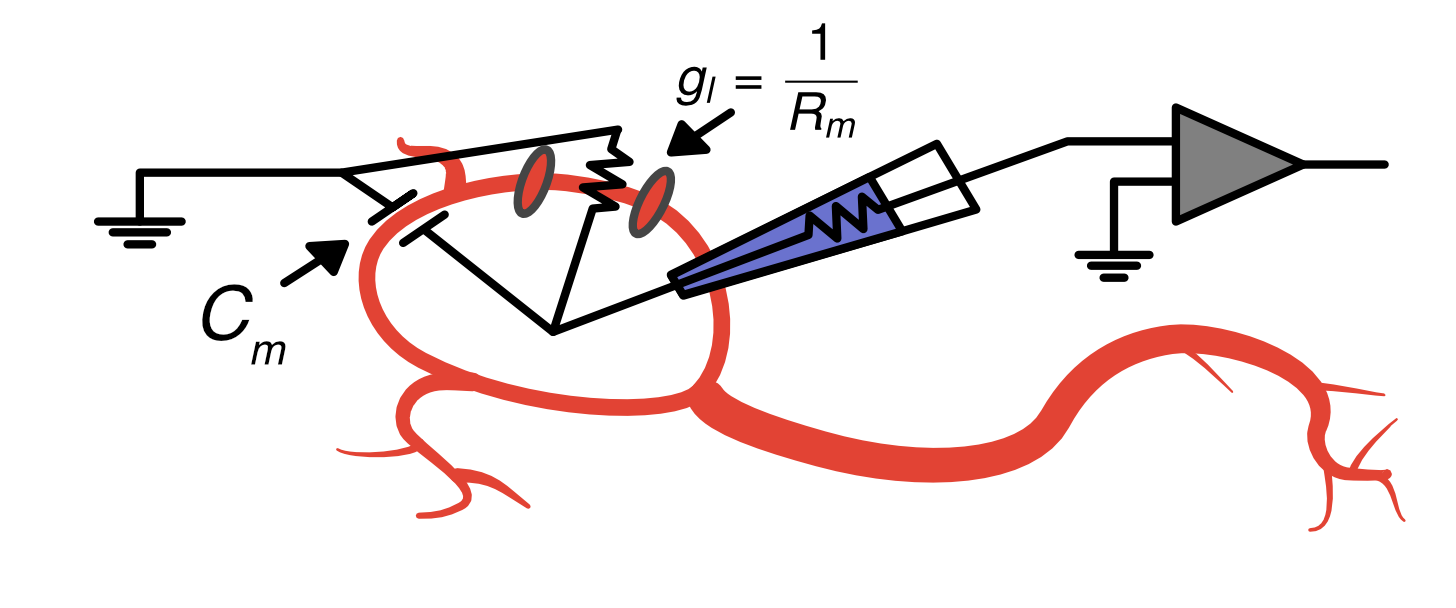
\includegraphics{img/GIF_circuit.png}
        \caption{Useful caption.}
        \label{fig:real_fig}
    \end{subfigure}
    \begin{subfigure}{0.22\textwidth}
        \includegraphics{example-image}
        \caption{Another caption.}
    \end{subfigure}
    \begin{subfigure}{0.3\textwidth}
        \includegraphics[height=1in]{example-image}
        \caption{One more caption.}
    \end{subfigure}
    \caption{Main figure caption.}
\end{figure}

